\section{V\_selector: A rotating velocity selector}
\label{vselector}
\index{Optics!Velocity selector}

%\component{V\_selector}{System}{$L_0$, $L_1$, $\omega$, $r_0$, $\phi$, $N$, height, width}{}{validated, position is center of input aperture}
\mcdoccomp{optics/V_selector.parms}

\begin{figure}
  \begin{center}
    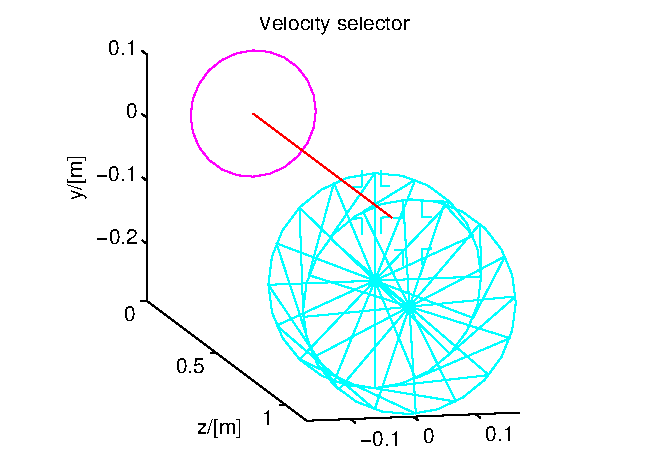
\includegraphics[width=0.9\textwidth]{figures/vselector}
  \end{center}
\caption{A velocity selector}
\label{f:vselector}
\end{figure}

The component {\bf V\_selector} models a rotating velocity
selector constructed from $N$ collimator blades
arranged radially on an axis. Two identical slits ($height \times width$)
at a 12 o'clock position allow
neutron passage at the position of the blades.
The blades are "twisted" on the axis so that a stationary
velocity selector does not transmit neutrons; the total
twist angle is denoted $\phi$ (in degrees).

Further input parameters for {\bf V\_selector} 
the distance between apertures, $L_0$, the length of the
collimator blades, $L_1$, the height from rotation axix to the slit
centre, $r_0$, the rotation speed $\omega$ (in rpm), 
and the blade thickness $t$.

The local coordinate system has its Origo at the slit centre.

The component {\rm Selector} produces equivalent results.

\subsection{Velocity selector transmission}

By rotating the selector you allow
transmittance of neutrons rays with velocities around a nominal value, given by
\begin{equation}
V_0 = \omega L / \phi ,
\end{equation}
which means that the selector has turned the twist angle
$\phi$ during the typical neutron flight time $L/V_0$. The actual twist angle
is $\phi' = \omega t = \omega L / V$.

Neutrons having a velocity slightly different from $V_0$
will either be transmitted or absorbed depending on the exact position
of the rotator blades when the neutron enters the selector.
Assuming this position to be unknown and integrating over all possible
positions (assuming zero thickness of blades), we arrive at a transmission factor
\begin{equation}
T = \left\{
 \begin{array}{ll}
 1 - (N/2\pi ) |\phi-\omega L / V| &
        {\rm if}\;   (N/2\pi )|\phi -\omega L / V| < 1 \\
    0  &  {\rm otherwise}
 \end{array} \right.
\end{equation}
where $N$ is the number of collimator blades.

A horisontal divergence changes the above formula because of the
angular difference between the entry and exit points of the neutron.
The resulting transmittance resembles the one above, only with
$V$ replaced by $V_z$ and $\phi$ replaced by $(\phi +\psi )$,
where $\psi$ is the angular difference due to
the divergence. An additional vertical divergence does not change
this formula, but it may contribute to $\psi$.
(We have here ignored the very small non-linearity of $\psi$ along the
neutron path in case of both vertical and horisontal divergence).

Adding the effect of a finite blade thickness, $t$, reduces the transmission
by the overall factor
\begin{equation}
\left( 1-\frac{N t}{2\pi r}  \right),
\end{equation}
where $r$ is the distance from the rotation axis. We ignore the variation
of $r$ along the neutron path and use just the average value.


